\documentclass{article}
\usepackage{mainPoly}

\title{Suites Numériques}
\author{Première Spécialité Mathématiques}
\date{}

\begin{document}
\maketitle
\section{Définition d'une suite}
\begin{tcolorbox}
\begin{definition}
Une \textbf{suite numérique réelle} est une fonction $u$ définie sur $\N$ à valeurs dans $\R$. Pour tout $n \in \N$, on note l'image $u(n)$ sous le format $u_n$, qui se lit \emph{\og $u$ indice $n$ \fg}. Cette image est appellée \textbf{terme de rang $n$ de $u$}.
\end{definition}
\end{tcolorbox}
\begin{example}
De nombreux phénomènes ne présentent pas de continuité, et peuvent être modélisés par des suites.
\begin{itemize}
\item Le chiffre d'affaire d'une entreprise $n$ mois après sa création.
\item Le nombre de façons de ranger $n$ figurines sur une étagère.
\item L'aire de la figure suivante après la $n$-ième étape.
\begin{center}
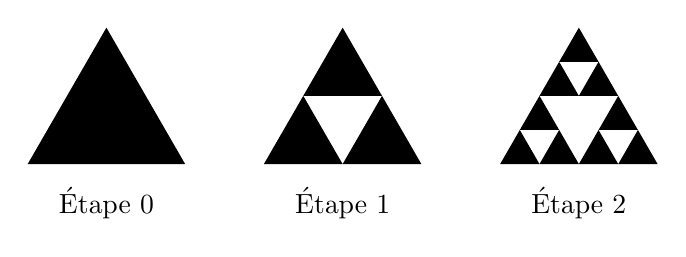
\begin{tikzpicture}
\fill (0,0) -- ++(0:2) -- ++(120:2);

\fill (3,0) -- ++(0:1) -- ++(120:1);
\fill (4,0) -- ++(0:1) -- ++(120:1);
\fill (3,0) ++(60:1) -- ++(0:1) -- ++(120:1);

\fill (6,0) -- ++(0:0.5) -- ++(120:0.5);
\fill (6.5,0) -- ++(0:0.5) -- ++(120:0.5);
\fill (7,0) -- ++(0:0.5) -- ++(120:0.5);
\fill (7.5,0) -- ++(0:0.5) -- ++(120:0.5);
\fill (6,0) ++ (60:0.5) -- ++(0:0.5) -- ++(120:0.5);
\fill (7,0) ++ (60:0.5) -- ++(0:0.5) -- ++(120:0.5);

\fill (6,0) ++ (60:1) -- ++(0:0.5) -- ++(120:0.5);
\fill (6,0) ++ (60:1) ++(0:0.5) -- ++(0:0.5) -- ++(120:0.5);
\fill (6,0) ++ (60:1) ++(60:0.5) -- ++(0:0.5) -- ++(120:0.5);

\draw (1,-0.5) node {Étape $0$};
\draw (4,-0.5) node {Étape $1$};
\draw (7,-0.5) node {Étape $2$};
\end{tikzpicture}
\end{center}
\end{itemize}
\end{example}
\begin{remark}
Une suite peut-être présentée sous la forme d'une séquence de nombres. Dans ce cas, le premier nombre de cette liste correspond au terme d'indice $0$.
\end{remark}
\begin{tcolorbox}
Pour parler d'une suite $u$ en toute généralité, on la note $(u_n)_{n \in \N}$.
\end{tcolorbox}
\begin{remark}
Ainsi, on ne confondra pas les notations $(u_n)_{n \in \N}$ (la suite en toute généralite) et $u_n$ (le $n$\ieme{} terme de la suite).
\end{remark}

\begin{definition}
Si l'on connait $f(n)$ une expression dépendant de $n$ telle que pour tout $n$, $u_n = f(n)$, alors on dit que la suite $(u_n)_{n \in \N}$ est définie de façon \textbf{explicite}.
\end{definition}
\begin{example}
Pour chacune des définitions explicites de $(u_n)_{n \in \N}$ données ci-dessous, donner les 4 premiers termes $u_0; u_1; u_2$ et $u_3$.
\begin{itemize}
\item $u_n = 3n + 1$ pour tout $n \in \N$ : \answersline
\item $u_n = 5 \times 2^n$ pour tout $n \in \N$ : \answersline
\item $u_n = \text{\og Le nombre de lettres dans l'écriture en français de $n$ \fg}$, pour tout $n \in \N$ : \answersline
\end{itemize}
\end{example}
\begin{tcolorbox}
\begin{definition}
Soit $(u_n)_{n \in \N}$ une suite numérique. On dit que $u_n$ est définie \textbf{par récurrence} si $u_0$ est connue, et si pour tout $n \in \N$, le terme $u_{n+1}$ est obtenu en fonction de $u_n$.  
\end{definition}
\end{tcolorbox}
\begin{example}
Pour chacune des définition par récurrence de $(v_n)_{n \in \N}$, calculer les $4$ premiers termes $v_0; v_1; v_2$ et $v_3$.
\begin{itemize}
\item $v_0 = 6$ et $v_{n+1} = v_n + 4$ : \answersline
\item $v_0 = 2$ et $v_{n+1} = 5 \times v_n$ : \answersline 
\end{itemize}
\end{example}
\newpage
\section{Étude de suites}
\subsection{Représentation graphique}
Soit $(u_n)_{n \in \N}$ une suite numérique. Pour représenter $(u_n)_{n \in \N}$ sur un repère orthonormé, on y fait figurer les points de coordonnées $(n;u_n)$.
\begin{center}
\includegraphics[width=\textwidth]{Repr_suite.png}
\end{center}
\subsection{Variation de suites}
\begin{tcolorbox}
\begin{definition}
Soit $(u_n)_{n \in \N}$ une suite numérique.
\begin{itemize}
\item On dit que $(u_n)_{n \in \N}$ est \textbf{croissante} si et seulement si pour tout $n \in \N$, on a $u_n \leq u_{n+1}$. 
\item On dit que $(u_n)_{n \in \N}$ est \textbf{décroissante} si et seulement si pour tout $n \in \N$, on a $u_{n+1} \leq u_n$. 
\end{itemize}
\end{definition}
\end{tcolorbox}
\begin{proposition}
Soit $(u_n)_{n \in \N}$ une suite numérique.
\begin{itemize}
\item La suite $(u_n)_{n \in \N}$ est croissante si et seulement si, pour tout $n \in \N$, $u_{n+1} - u_n \geq 0$. 
\item La suite $(u_n)_{n \in \N}$ est décroissante si et seulement si, pour tout $n \in \N$, $u_{n+1} - u_n \leq 0$. 
\end{itemize}
\end{proposition}
\begin{example}
Étudier les variations des suites suivantes :
\begin{enumquestions}
\item $(u_n)_{n \in \N}$ définie par $u_n = 8 + 4n$ pour tout $n \in \N$.
\item $(v_n)_{n \in \N}$ définie par $v_0 = 64$ et $v_{n+1} = \dfrac{v_n}{2}$ pour tout $n \in \N$.
\item $(w_n)_{n \in \N}$ définie par $w_n = \dfrac{n}{n+1}$ pour tout $n \in \N$.
\item $(z_n)_{n \in \N}$ définie par $z_n = (-1)^n$ pour tout $n \in \N$.
\end{enumquestions}
\emptybox{6cm}
\end{example}
\end{document}